\chapter{Magnetismo de sólidos} \label{Ch:10}

\section{Relaciones básicas}

\section{Diamagnetismo atómico}

\section{Paramagnetismo atómico}

\section{Paramagnetismo de los electrones de conducción}

\section{La interacción de intercambio}

\section{Ferromagnetismo}

\section{Dominios ferromagnéticos}

\section{Orden ferrimangético}
\begin{figure}[h!] \centering
	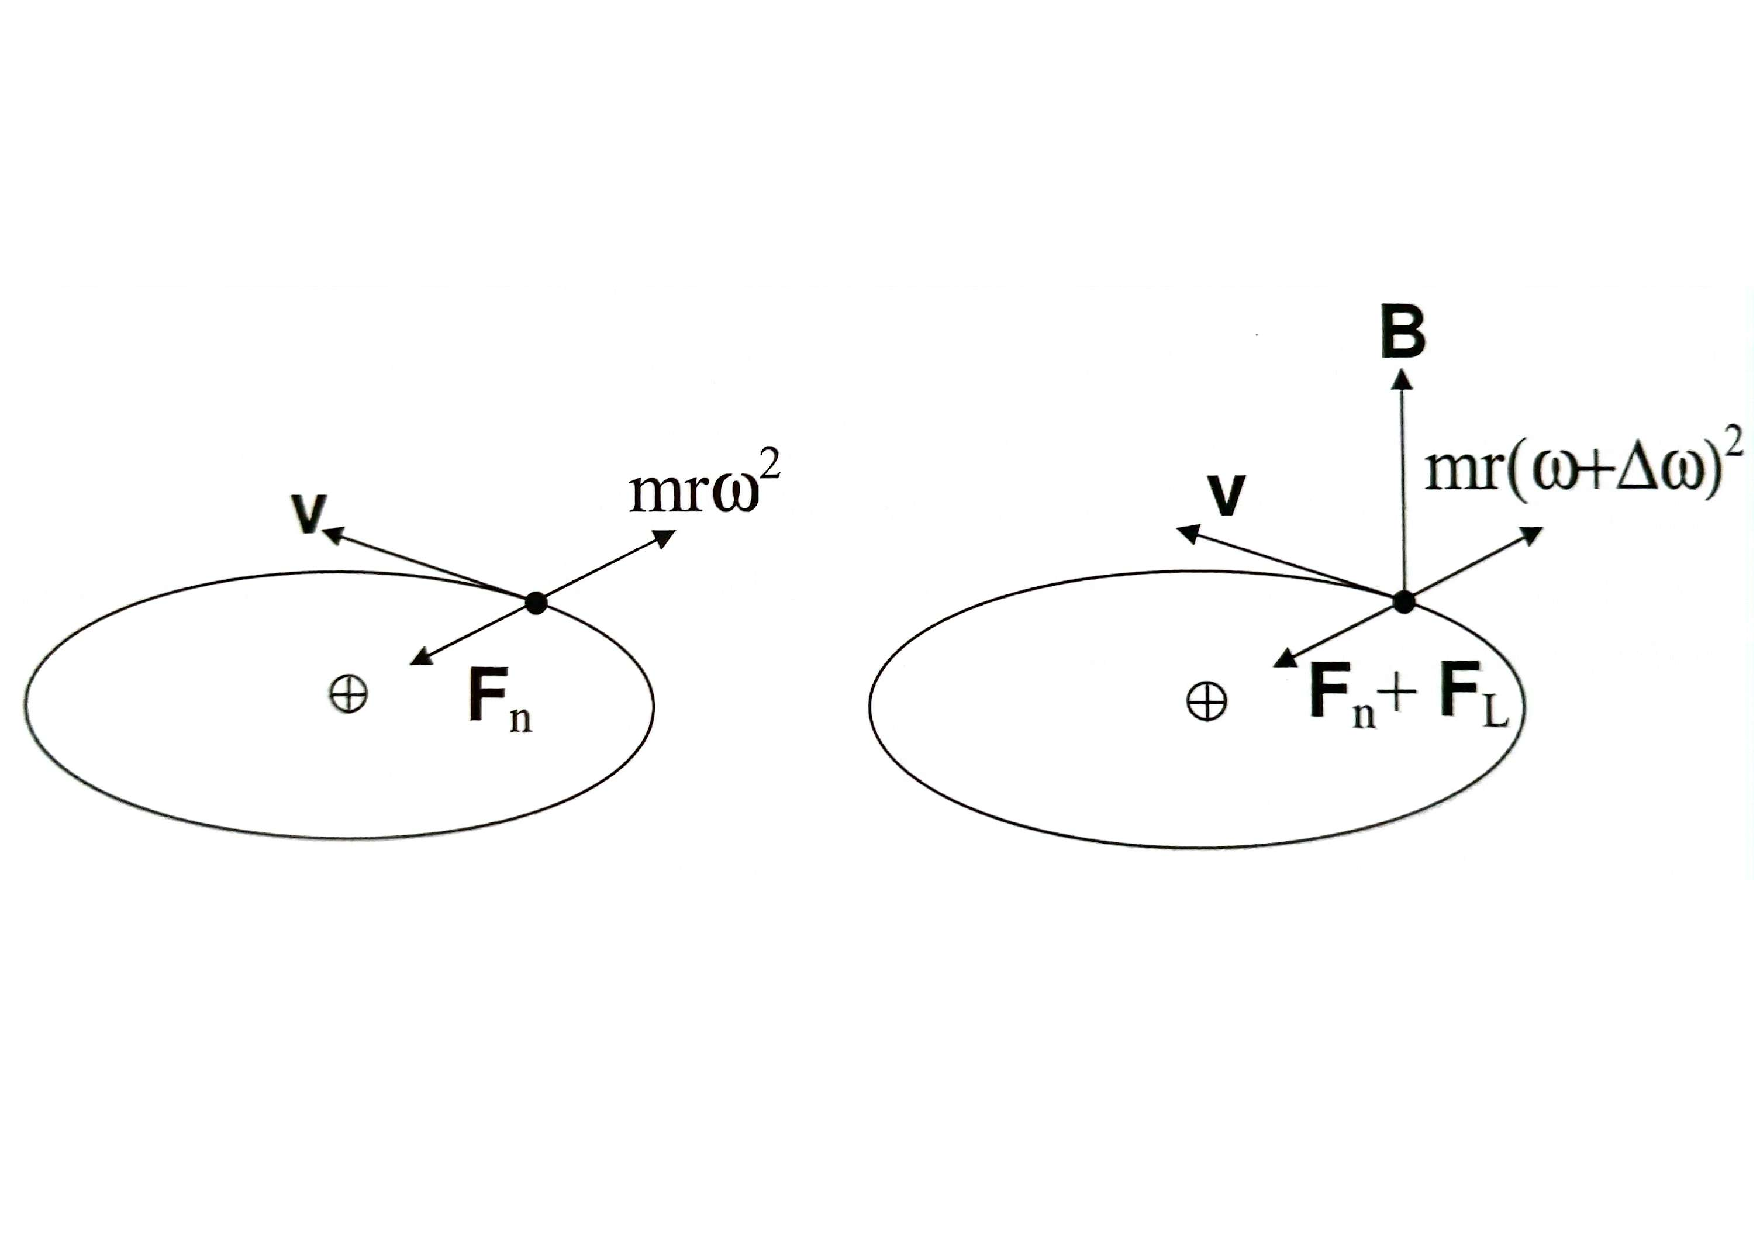
\includegraphics[scale=0.5]{Cuerpo/Ch_10/Fotos libro 1.pdf}
	\caption{}
	\label{Fig:10-01}
\end{figure}
\begin{figure}[h!] \centering
	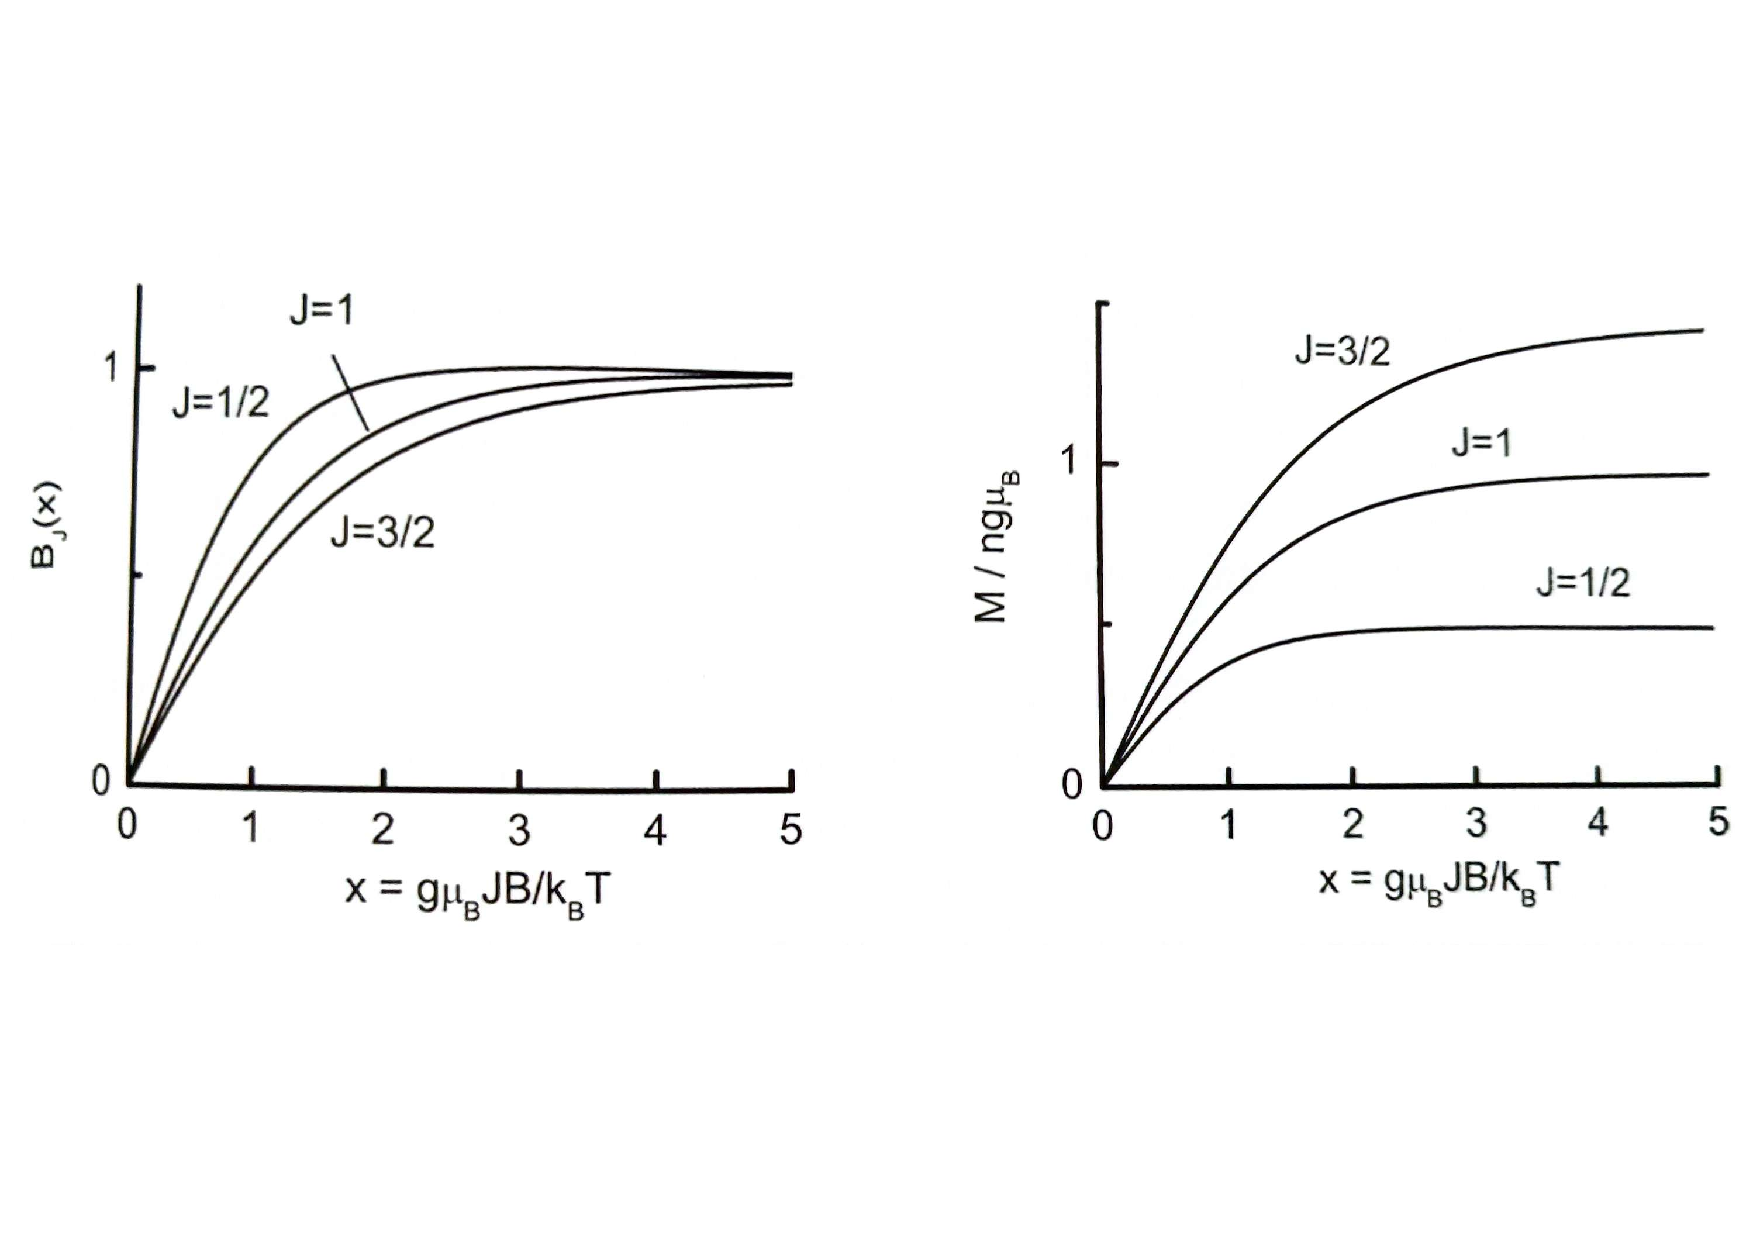
\includegraphics[scale=0.5]{Cuerpo/Ch_10/Fotos libro 2.pdf}
	\caption{}
	\label{Fig:10-02}
\end{figure}
\begin{figure}[h!] \centering
	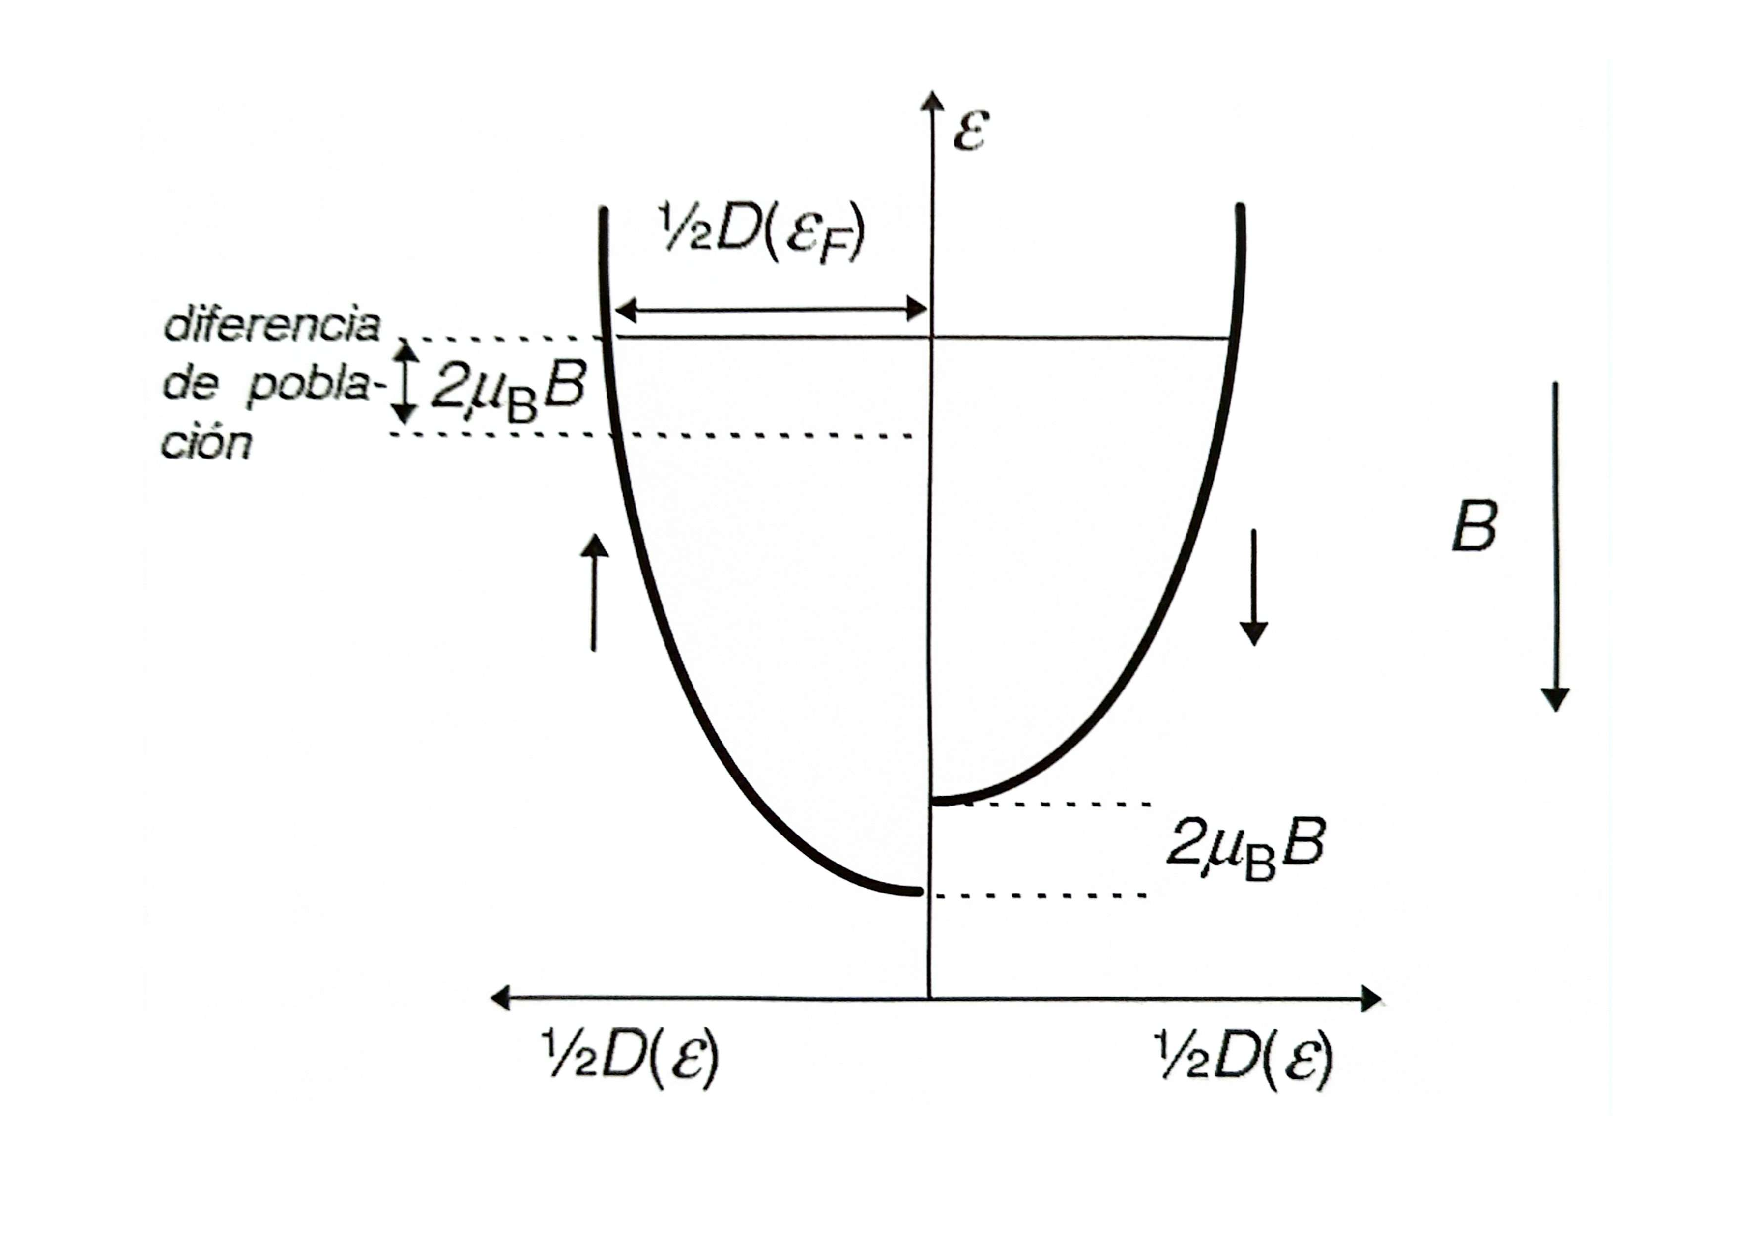
\includegraphics[scale=0.5]{Cuerpo/Ch_10/Fotos libro 3.pdf}
	\caption{}
	\label{Fig:10-03}
\end{figure}
\begin{figure}[h!] \centering
	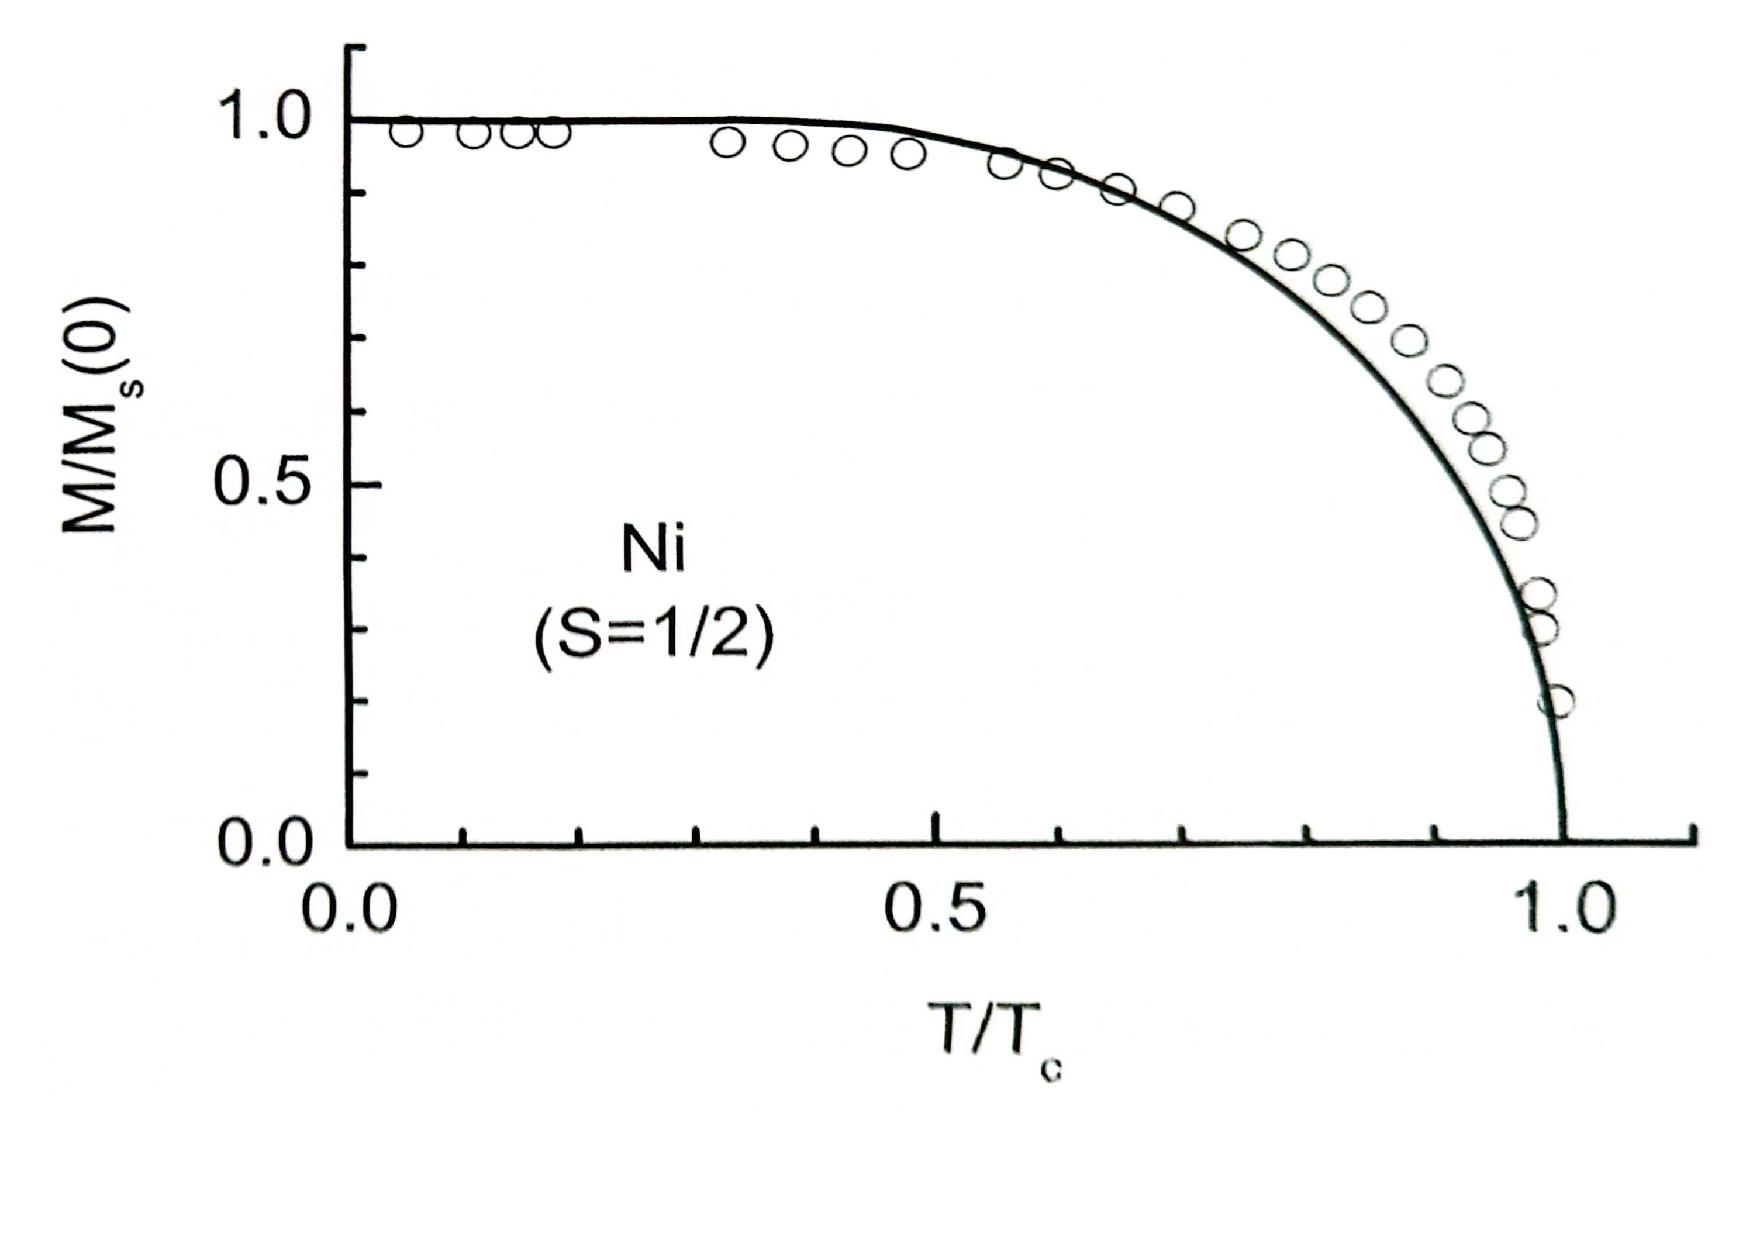
\includegraphics[scale=0.5]{Cuerpo/Ch_10/Fotos libro 4.pdf}
	\caption{}
	\label{Fig:10-04}
\end{figure}
\begin{figure}[h!] \centering
	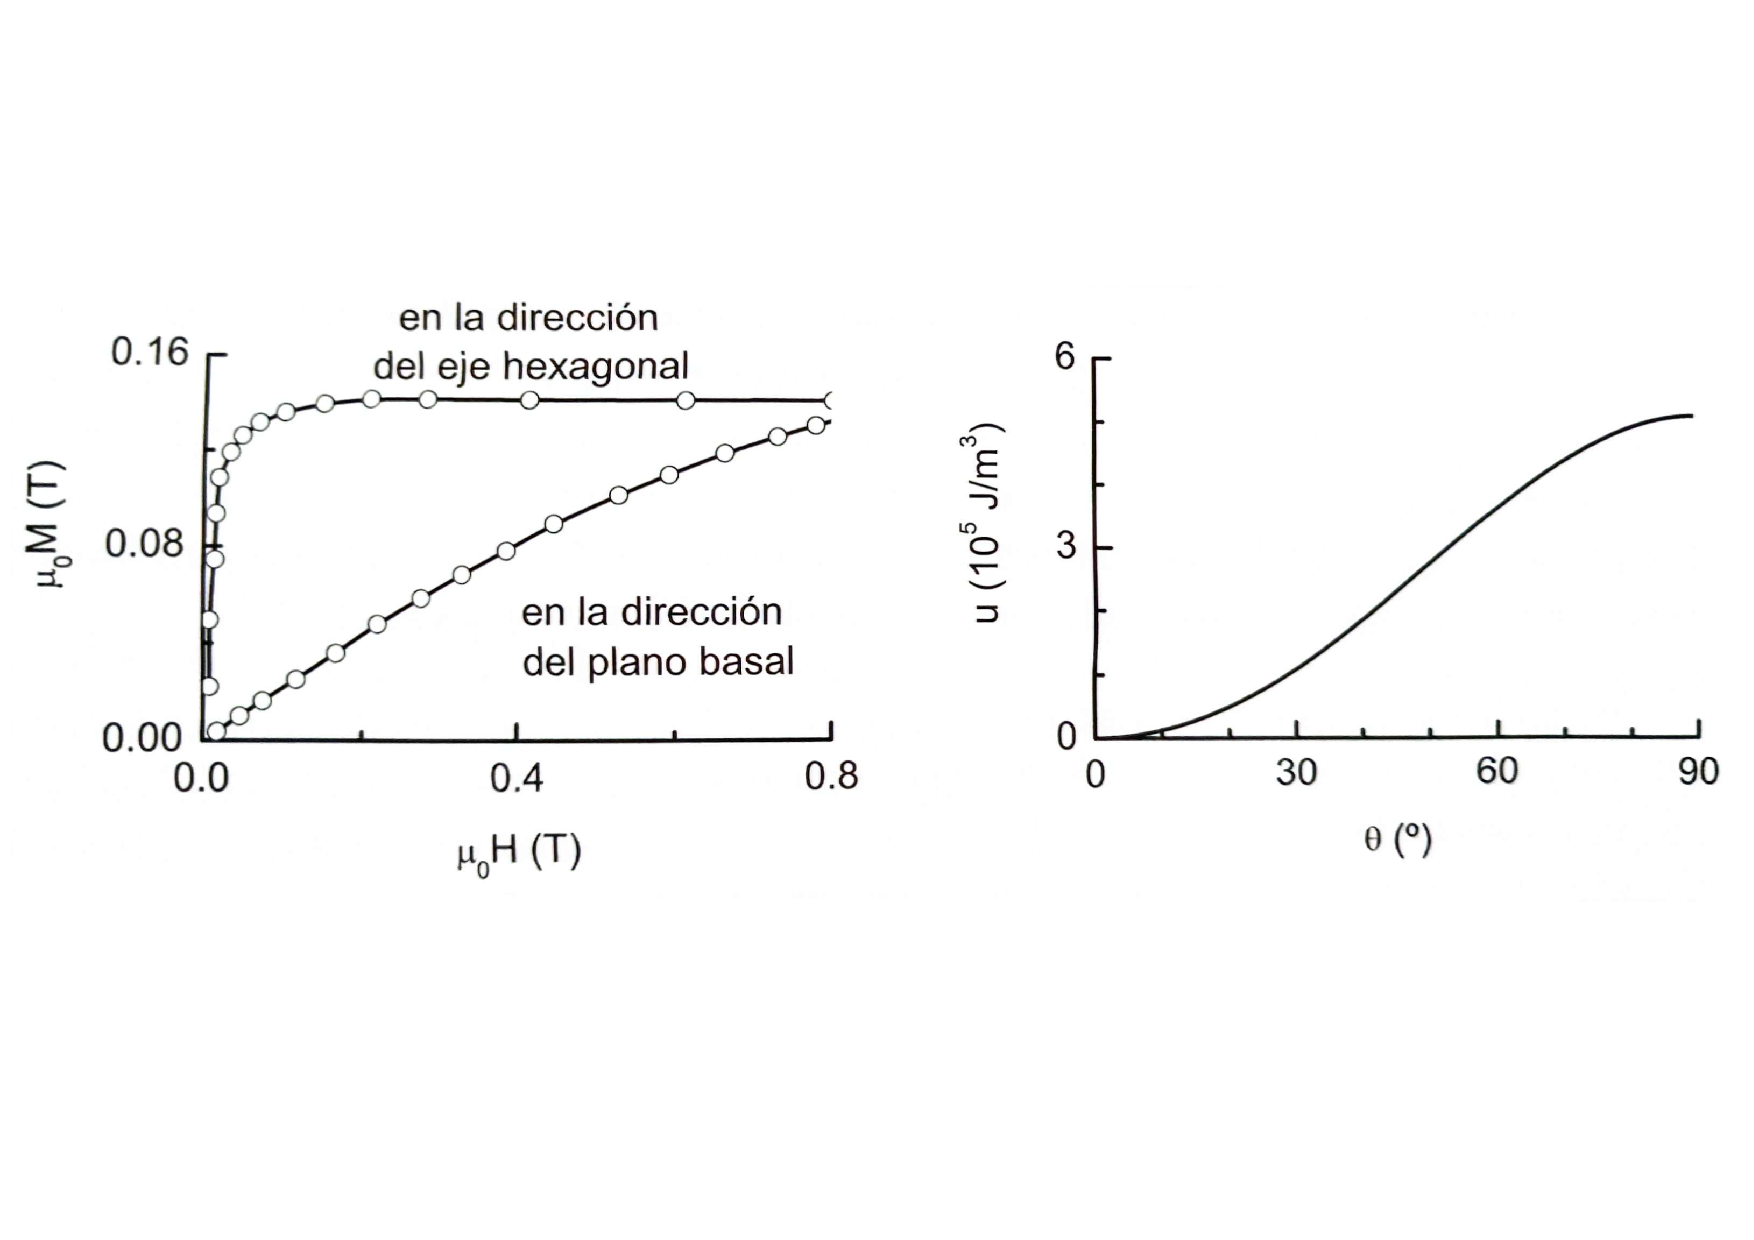
\includegraphics[scale=0.5]{Cuerpo/Ch_10/Fotos libro 5.pdf}
	\caption{}
	\label{Fig:10-05}
\end{figure}
\begin{figure}[h!] \centering
	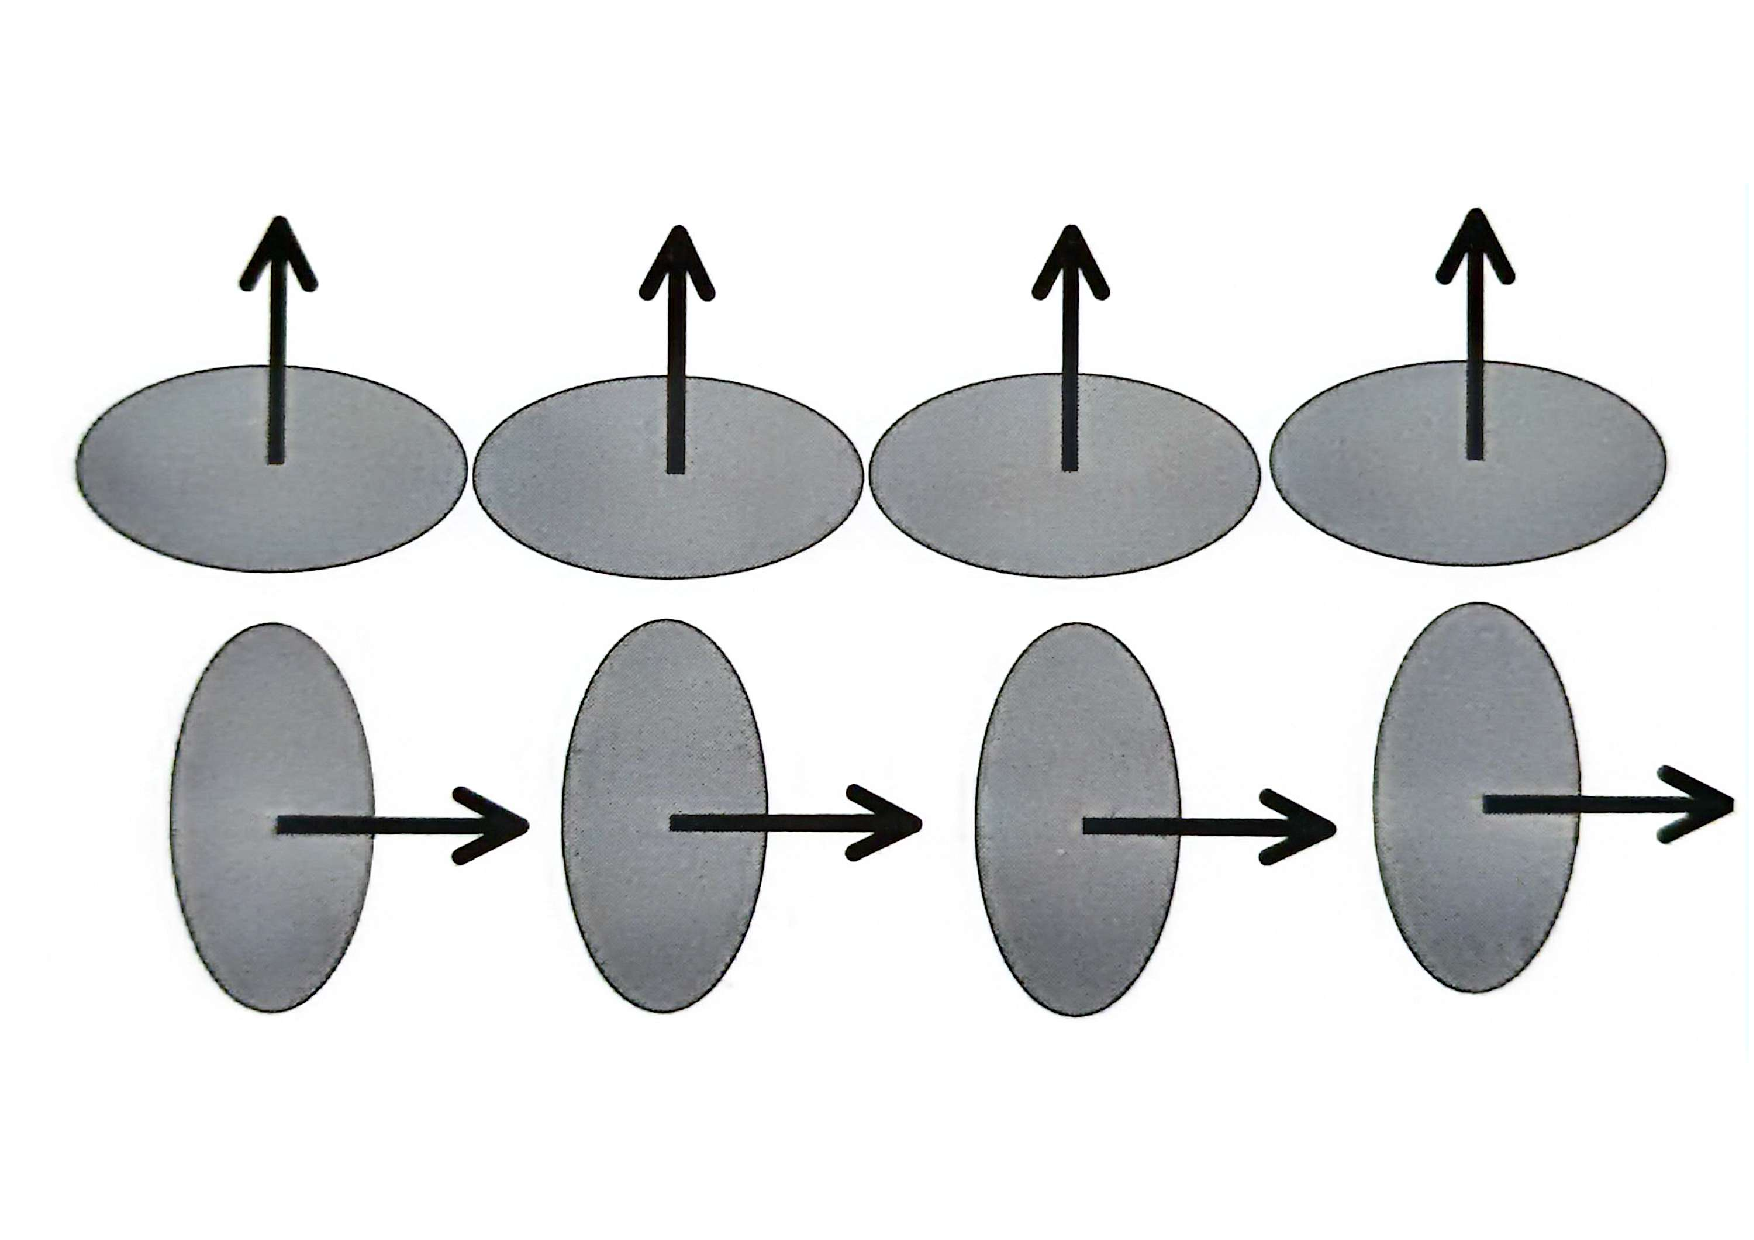
\includegraphics[scale=0.5]{Cuerpo/Ch_10/Fotos libro 6.pdf}
	\caption{}
	\label{Fig:10-06}
\end{figure}
\begin{figure}[h!] \centering
	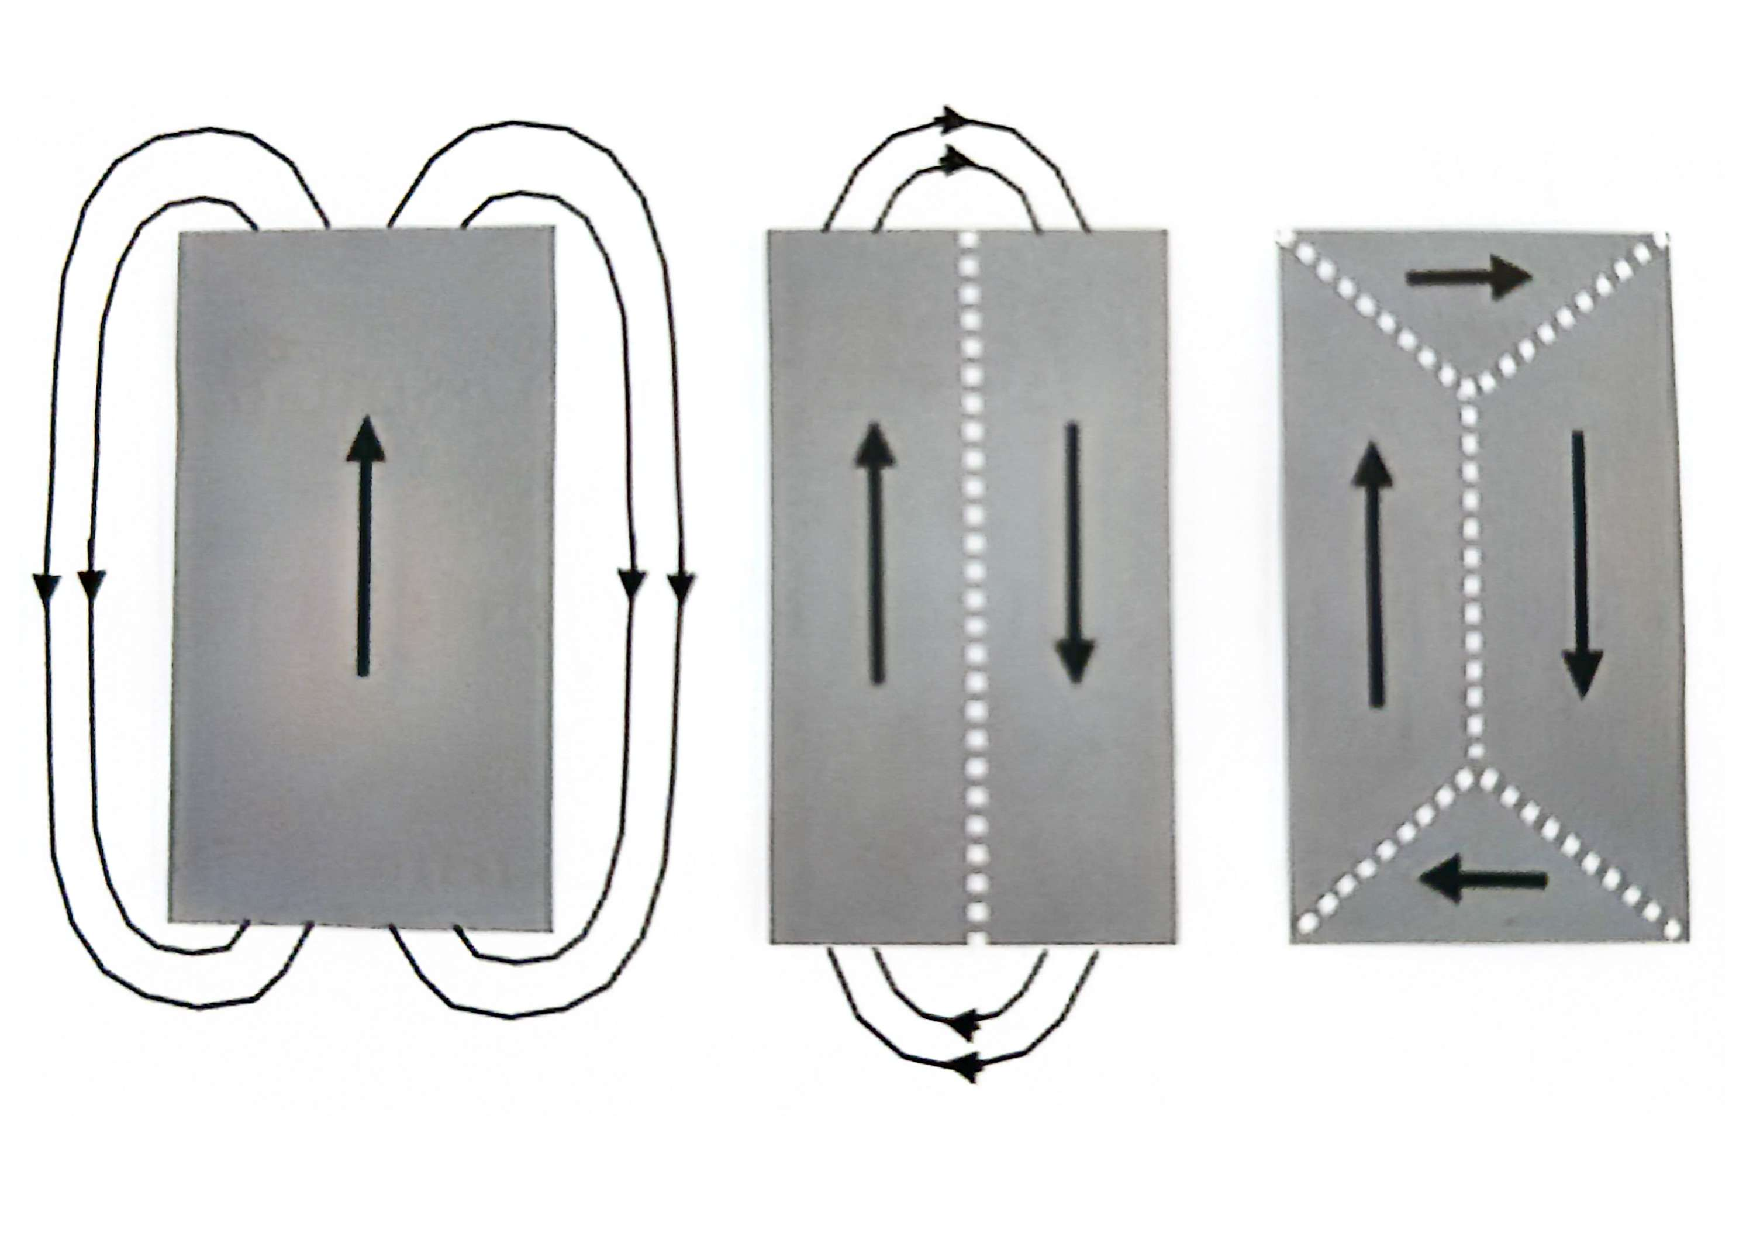
\includegraphics[scale=0.5]{Cuerpo/Ch_10/Fotos libro 7.pdf}
	\caption{}
	\label{Fig:10-07}
\end{figure}
\begin{figure}[h!] \centering
	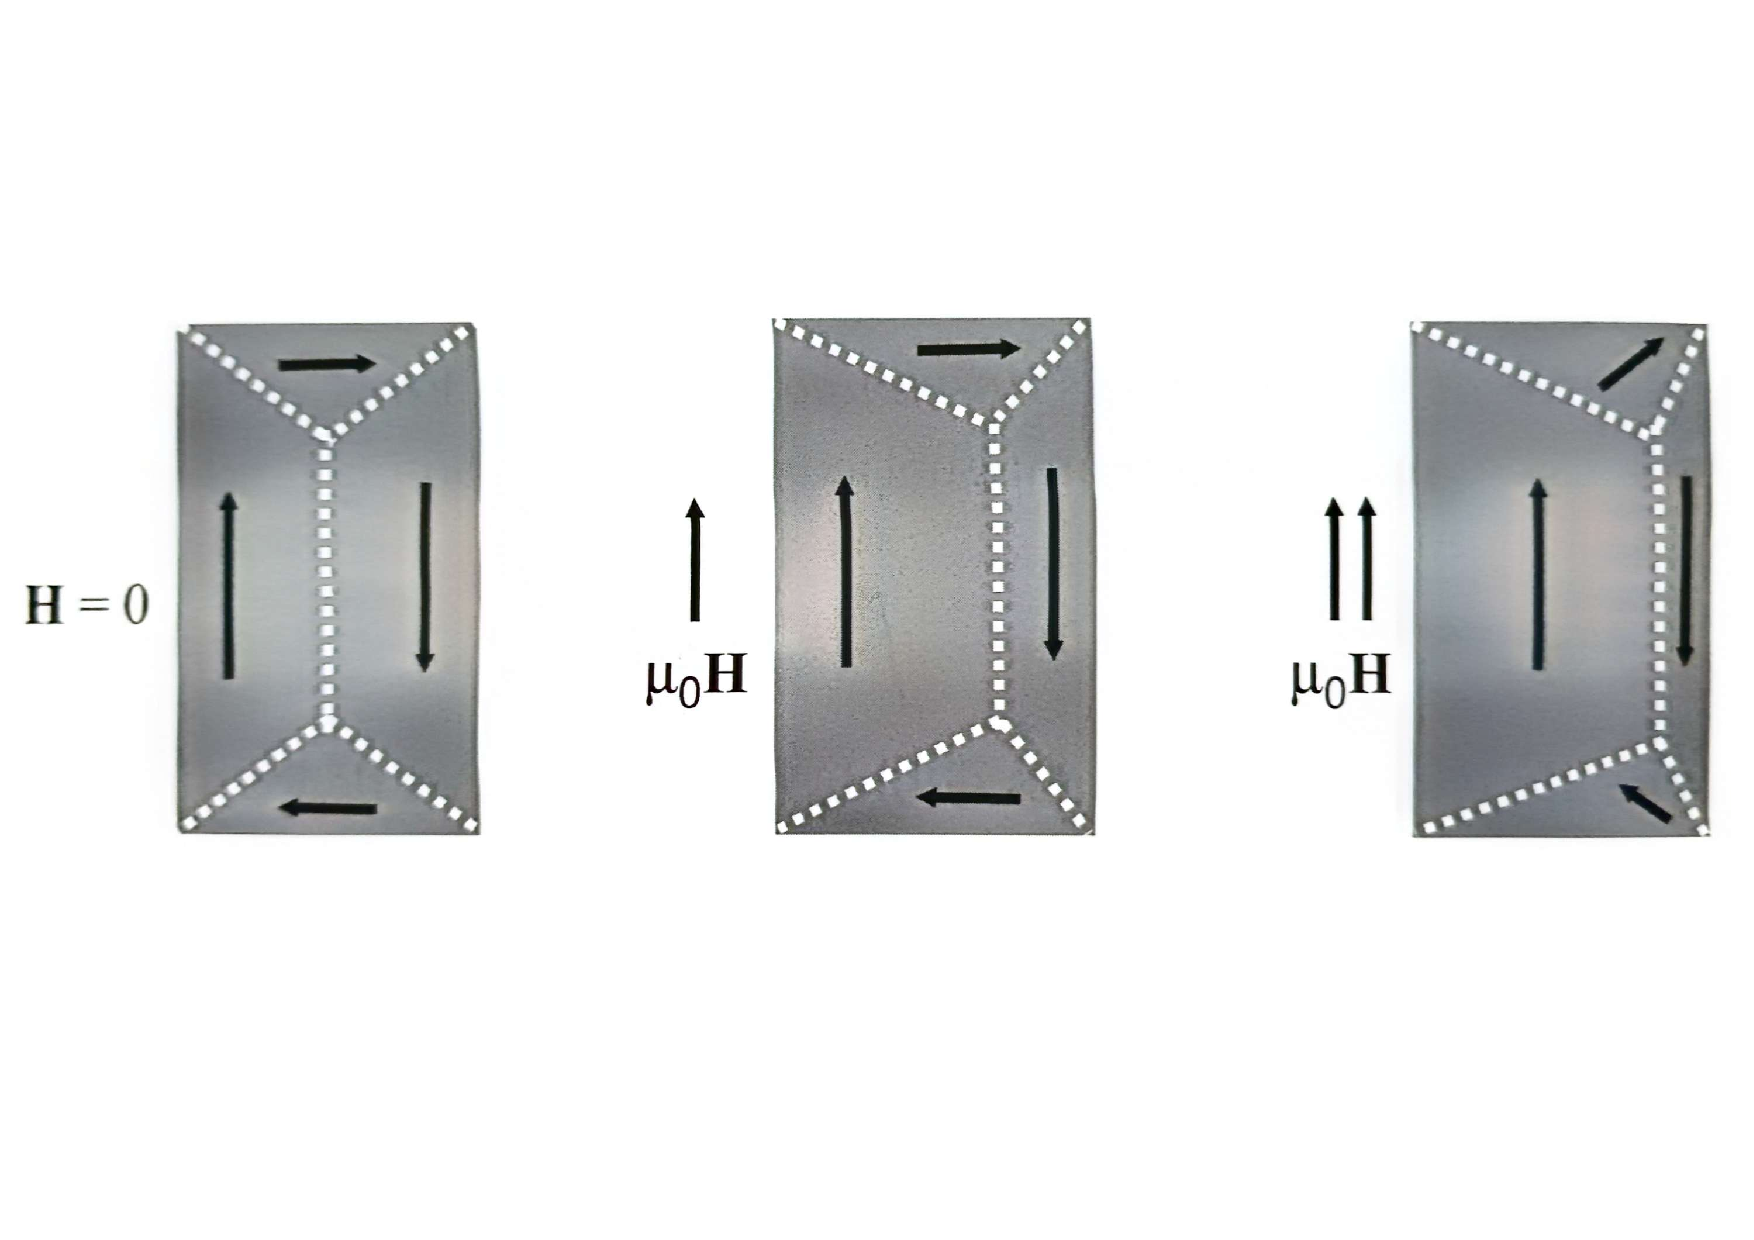
\includegraphics[scale=0.5]{Cuerpo/Ch_10/Fotos libro 8.pdf}
	\caption{}
	\label{Fig:10-08}
\end{figure}
\begin{figure}[h!] \centering
	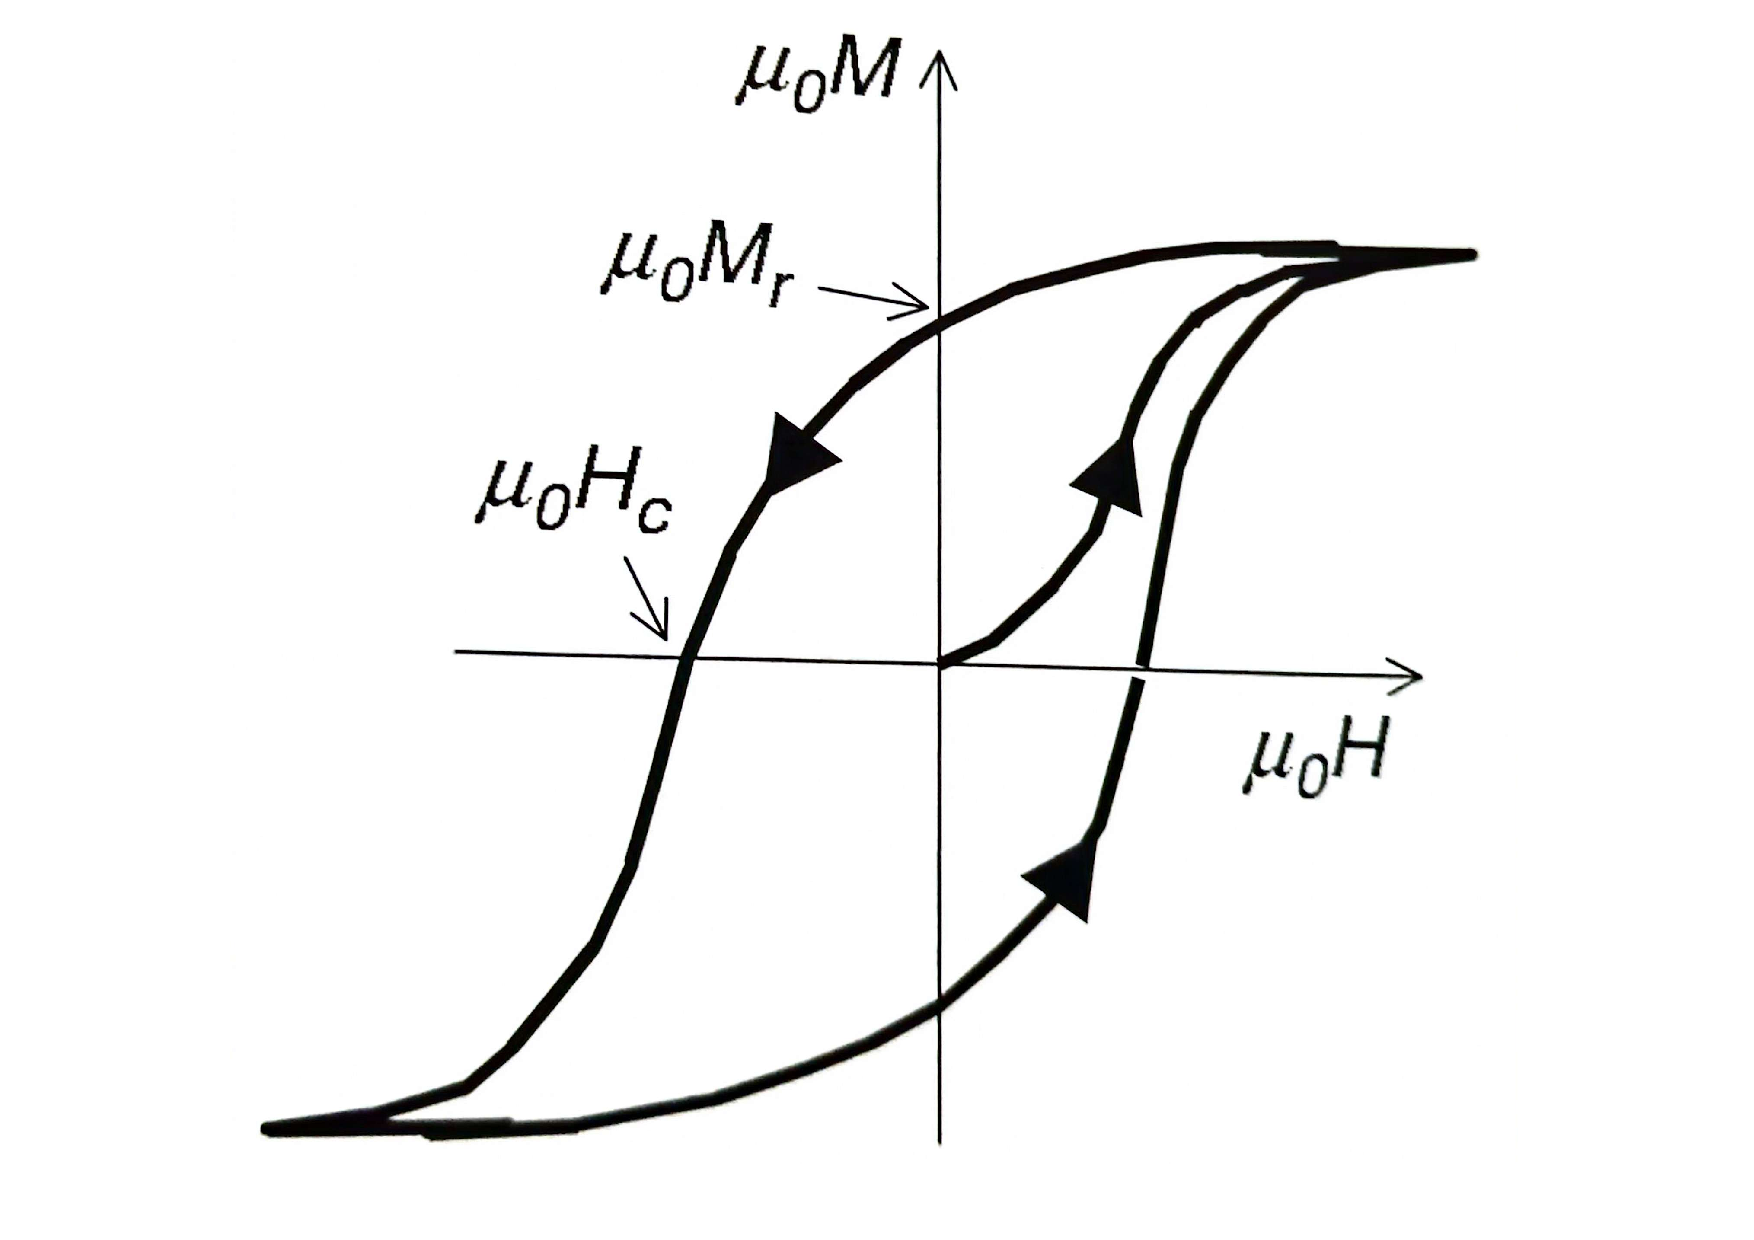
\includegraphics[scale=0.5]{Cuerpo/Ch_10/Fotos libro 9.pdf}
	\caption{}
	\label{Fig:10-09}
\end{figure}